\chapter{مدل طلایی}
\section{مقدمه}
در مدل‌ طلایی ۴ نوع متفاوت از \lr{Skein hash} آورده شده‌است (‌ ۲۲۴ و ۲۵۶ و ۳۸۴ و ۵۱۲  بیت) که همانطور که در مدل  طراحی شده با \lr{verilog} نیز تنها نوع استاندارد  (۵۱۲ بیت)آن پیاده‌سازی شده است , در مدل‌ طلایی نیز تنها توضیحات و مستندات این نوع ارائه خواهد شد.
\\
\begin{center}
	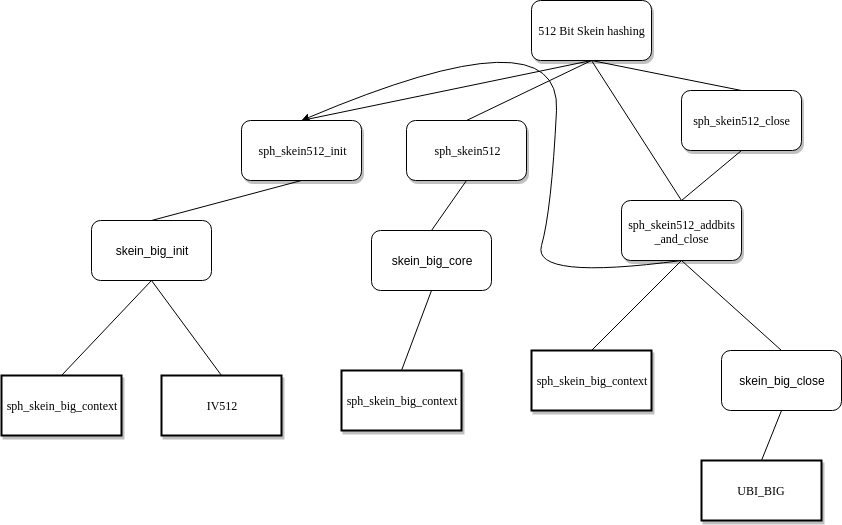
\includegraphics[width=14cm]{images/GoldenModel.png}
\end{center}

\section{پیاده‌سازی الگوریتم}
در شکل بالا تمامی توابع و ساختارهای مورد نیاز  و سلسله مراتب آن‌ها برای نوع ۵۱۲ بیتی الگوریتم آورده شده است , برای توضیح نحوه‌ی اجرای الگوریتم با شروع از  
\lr{sph-skein-big-context} سلسله اجرای برنامه توضیح داده خواهد شد.
\\
در این برنامه برای ‌ذخیره و استفاده از هش , از ساختاری استفاده شده است به نام \hyperref[subsec:sph-skein-big-context]{\lr{sph-skein-big-context}} استفاده شده است و هدف برنامه اجرای الگوریتم هش و ذخیره‌ی خروجی در این ساختار است.
\\
برای اجرای الگوریتم هش ۵۱۲ بیتی , در سلسله‌ی اجرا از توابع زیر استفاده شده است :
\\
در ابتدا برنامه با ذخیره‌ی مقادیر از پیش تعیین شده  \hyperref[subsec:IV512]{\lr{IV512}} در ساختار معرفی شده شروع به کار می‌کند , و این کار توسط تابع\\
\hyperref[subsec:sph-skein512-init]{\lr{sph-skein512-init}}
  انجام میگردد.
  \\ سپس با در نظر گرفتن ورودی و سایز این ورودی، اجرای الگوریتم هش  توسط تابع \hyperref[subsec:sph-skein512]{\lr{sph-skein512}}
   شروع می‌شود و ورودی داده شده تبدیل به هش میشود و با ذخیره شدن در ساختار  هش، این تابع پایان می‌پذیرد.
  \\ 
  
  

